\documentclass[a4paper,fleqn]{cas-dc}

%%%Author definitions
\def\tsc#1{\csdef{#1}{\textsc{\lowercase{#1}}\xspace}}
\tsc{WGM}
\tsc{QE}
\tsc{EP}
\tsc{PMS}
\tsc{BEC}
\tsc{DE}
%%%

\usepackage[square,numbers,sort&compress,comma]{natbib}

\usepackage{amsmath}
\usepackage{amssymb}
\usepackage{diagbox}
\usepackage{caption}
\usepackage{graphicx}
\usepackage{latexsym}
\usepackage{times}
\usepackage[pagewise]{lineno}
\graphicspath{{figures/}}
\usepackage{color, colortbl}
\usepackage{chemformula}
\usepackage{xcolor}
\definecolor{Gray}{gray}{0.9}
\newcommand{\highlight}[1]{%
  \colorbox{Gray}{$\displaystyle#1$}}
\usepackage{color, colortbl}
\usepackage{chemformula}
\usepackage{xcolor}
\usepackage{adjustbox}
\usepackage{mathrsfs}
\usepackage{booktabs}
\usepackage{hyperref}
\usepackage{lipsum}

\emergencystretch = 0 pt
\pretolerance = 150
\tolerance = 250
\hbadness = 150
\hfuzz = 0 pt
\vfuzz = 0 pt

\newcommand{ \kamila}[1]{\color{blue}{Kamila: #1} \color{black}}
\newcommand{ \todump}[1]{\color{olive}{#1} \color{black}}
\usepackage[normalem]{ulem}

\begin{document}

\shorttitle{\texttt{pykitPIV}: PyTorch-compatible synthetic image generation for training flow estimation algorithms in particle image velocimetry}
\shortauthors{Zdyba\l{} et~al.}


\title [mode = title]{\texttt{pykitPIV}: PyTorch-compatible synthetic image generation for training flow estimation algorithms in particle image velocimetry}

\author[EMPA]{Kamila Zdyba\l{}*}
\ead{kamila.zdybal@gmail.com}

\author[EMPA]{Claudio Mucignat}
\author[EMPA]{Ivan Lunati}

\address[EMPA]{Laboratory for Computational Engineering, Swiss Federal Laboratories for Materials Science and Technology, Empa, Dübendorf, Switzerland}

\begin{abstract} 
We describe pykitPIV

\lipsum[60]
\end{abstract}

\begin{keywords}
particle image velocimetry; flow estimation; convolutional neural networks; Python
\end{keywords}

\maketitle

\section{Introduction\label{sec:introduction}}

\lipsum









\section{Software overview} \label{sec:software}



%\begin{figure}[t]
%\centering
%\includegraphics[width=7cm]{}
%\caption{}
%\label{fig:pykitPIV-modules}
%\end{figure}

\begin{figure*}[t]
\centering
\vspace{-0.4 in}
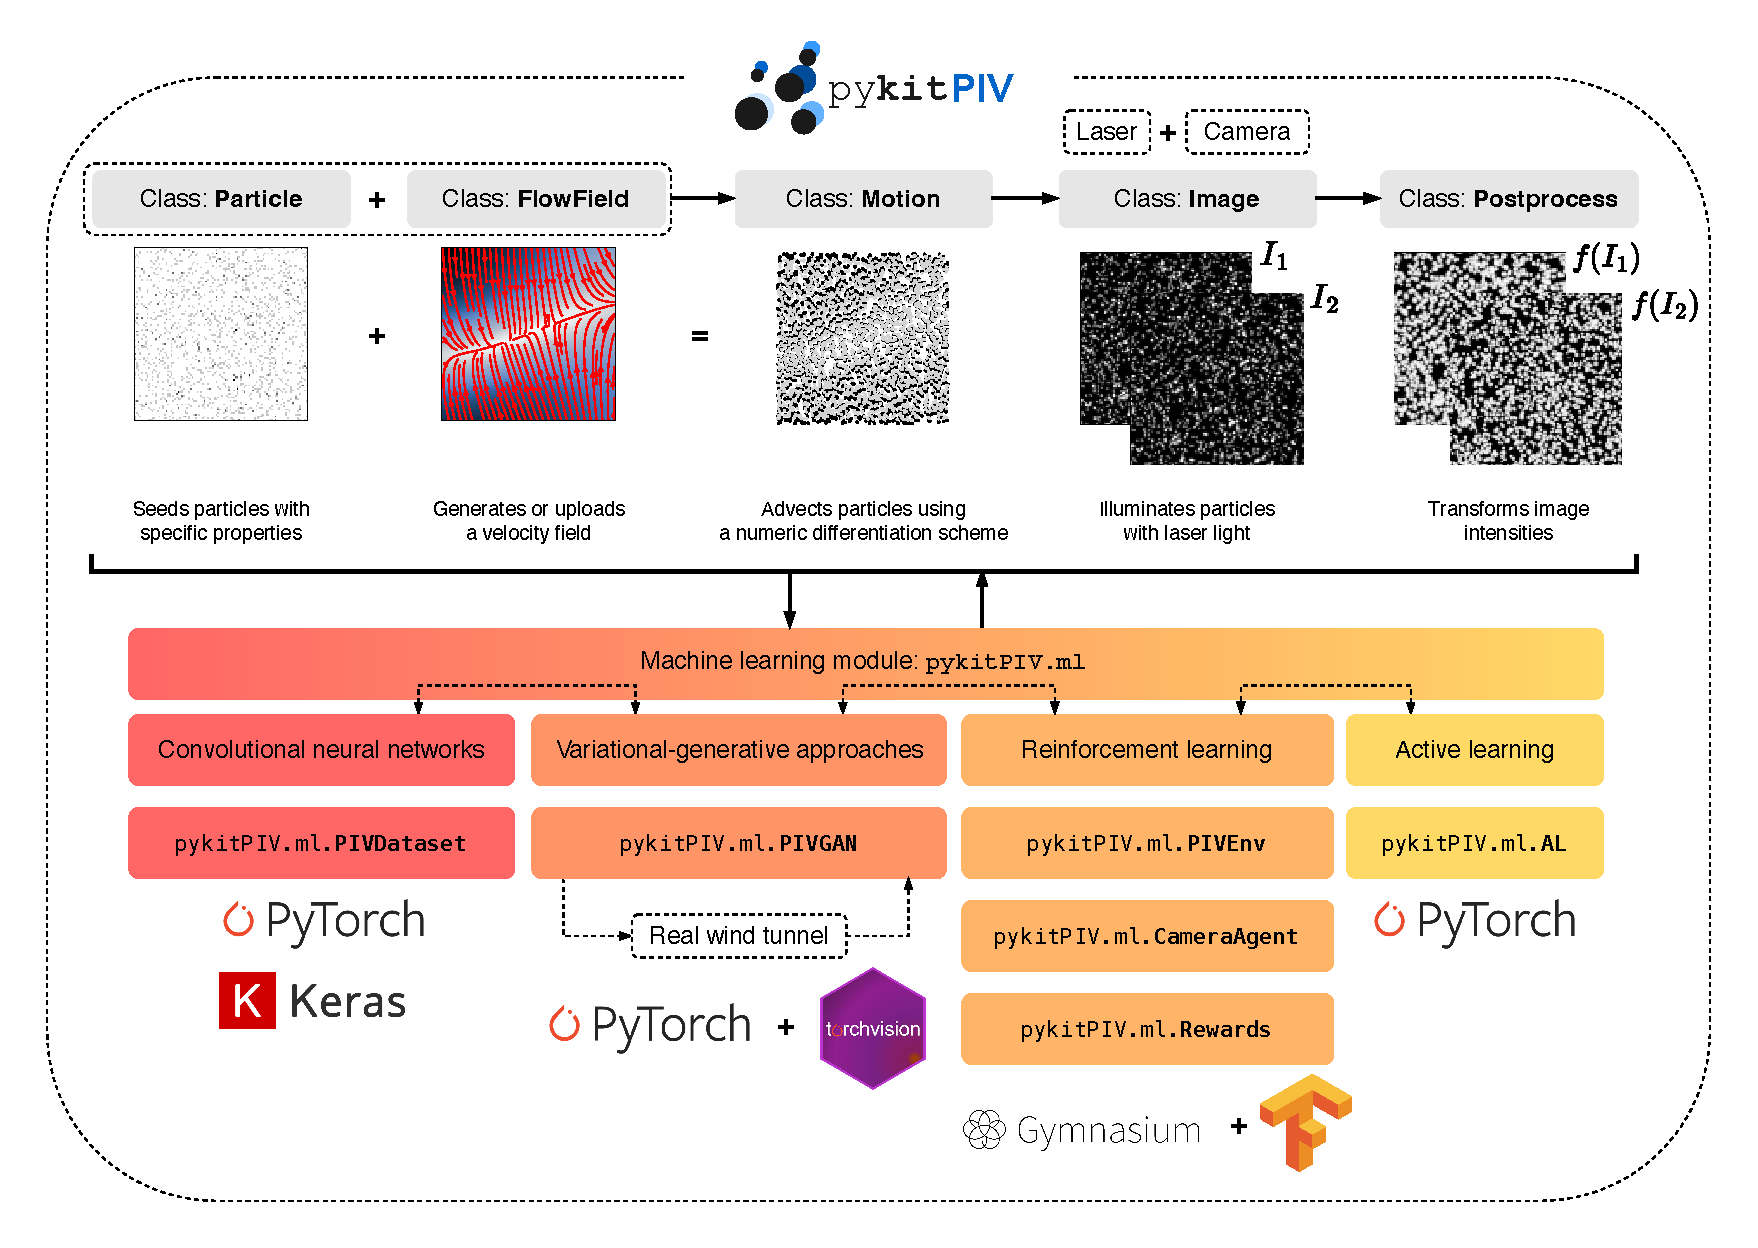
\includegraphics[width=\textwidth]{pykitPIV-modules.pdf}
\vspace{10 pt}
\caption{\footnotesize Order of using \texttt{pykitPIV} classes. At each stage of synthetic image generation, the user has freedom in selecting various parameters that would normally be available in an experimental setting such as particle seeding density, thickness of the laser plane, camera exposure, particle loss due to out-of-plane movement, or time separation between images.}
\label{fig:operations}
\end{figure*}

The PIV image pair tensor has shape $(N, 2, H, W)$, where $N$ is the batch size, $H$ is image height and $W$ is image width. The second dimension can be thought of as the number of channels and those correspond to $I_1$ and $I_2$, respectively. This is compatible with tensor shape accepted by convolutional layers implemented in PyTorch.






\section{Discussion} \label{sec:results}

\lipsum

%
%\begin{figure*}[t]
%\centering
%\vspace{-0.4 in}
%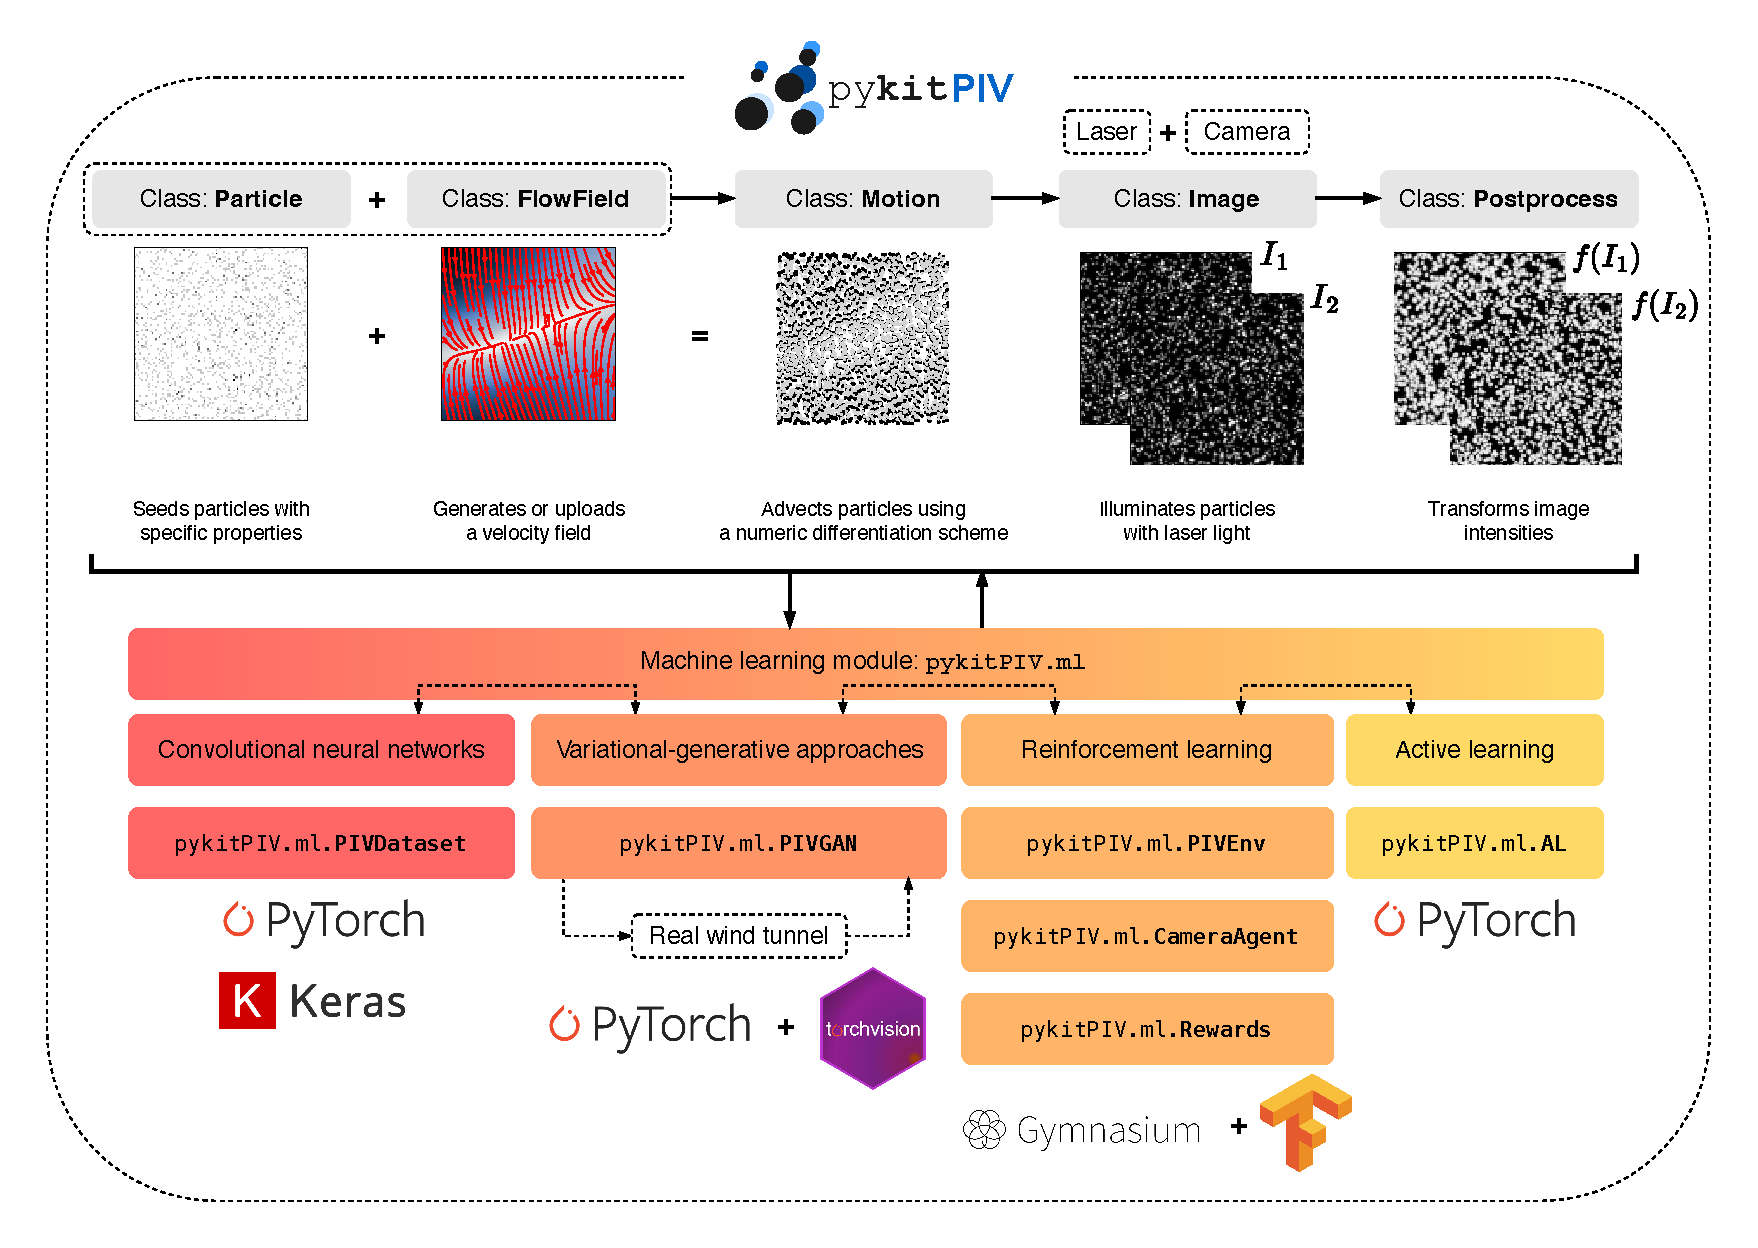
\includegraphics[width=\textwidth]{pykitPIV-modules.pdf}
%\vspace{10 pt}
%\caption{\footnotesize The variety of operations on PIV images possible with the pykitPIV modules.}
%\label{fig:operations}
%\end{figure*}


\section{Conclusions}



\section*{Declaration of competing interest}

The authors declare that they have no known competing financial interests or personal relationships that could have appeared to influence the work reported in this paper.

\section*{Author contributions}



\section*{Acknowledgments}




\bibliographystyle{pci}
\bibliography{bibliography}

\end{document}